\documentclass[12pt]{article}
\usepackage{graphicx}
\usepackage{hyperref}
\graphicspath{ {./images/} }
\usepackage[rightcaption]{sidecap}
\usepackage{subcaption}
\usepackage{wrapfig}
\usepackage{float}
\usepackage{ragged2e}
\usepackage{imakeidx}
\makeindex
\usepackage{listings}
\usepackage{xcolor}  % Required for defining colors
\usepackage[numbers,sort&compress]{natbib} 

% Define colors for the background of the code blocks
\definecolor{codegray}{gray}{0.9}
\definecolor{codewhite}{rgb}{1,1,1}

% Configure the appearance of the code blocks for Python
\lstdefinestyle{python}{
    backgroundcolor=\color{codegray},
    basicstyle=\ttfamily\small,  % Font and size of the code
    breaklines=true,             % Allow line breaks within the code
    frame=single,                % Add a border around the code block
    language=Python,             % Specify the Python language
    numbers=left,                % Display line numbers on the left
    numberstyle=\tiny\color{gray},  % Style for line numbers
    keywordstyle=\color{blue},       % Style for keywords
    commentstyle=\color{green!40!black},  % Style for comments
    stringstyle=\color{orange},           % Style for strings
}

% Configure the appearance of the code blocks for Bash
\lstdefinestyle{bash}{
    backgroundcolor=\color{codewhite},
    basicstyle=\ttfamily\small,  % Font and size of the code
    breaklines=true,             % Allow line breaks within the code
    frame=single,                % Add a border around the code block
    language=bash,               % Specify the Bash language
    numbers=left,                % Display line numbers on the left
    numberstyle=\tiny\color{gray},  % Style for line numbers
    keywordstyle=\color{blue},       % Style for keywords
    commentstyle=\color{green!40!black},  % Style for comments
    stringstyle=\color{orange},           % Style for strings
}
\title{ARGO}
\author{E. C. Semidalas and C. E. Semidalas}
\date{} % Remove the date

\begin{document}
\begin{titlepage}
    \centering
    {\Huge ARGO} \par
    \vspace{1cm} % Add space between title and author
    \vspace{1cm} % Add more space if needed
    {\Large Users Manual\\Version 1.3} \par
    \vspace{1cm} % Add more space if needed
    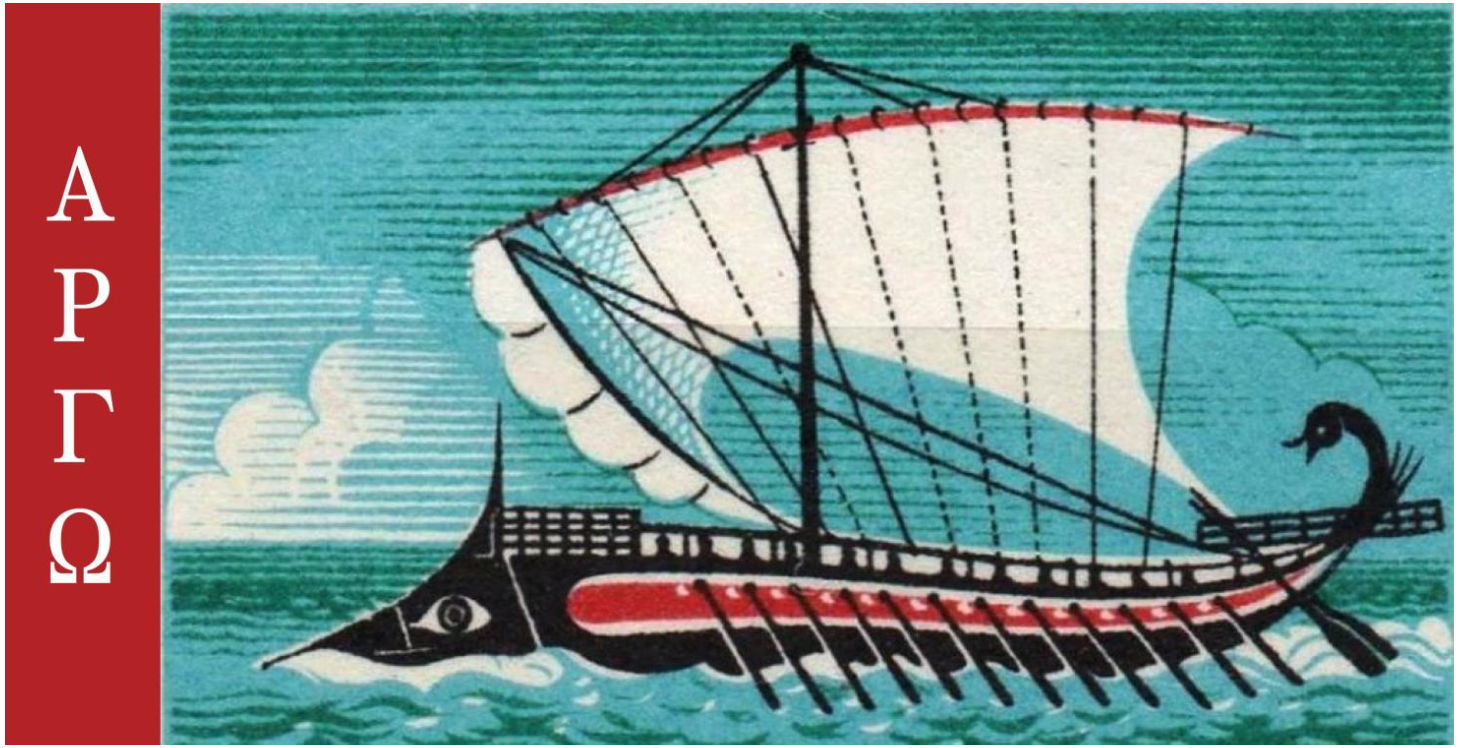
\includegraphics[width=0.50\textwidth]{argo_triiris.png} \par
    \label{fig1}
    \vspace{1cm} % Add space after the figure
    {\large \today} \par % Date information
    \vspace{1cm}    
    {E. C. Semidalas and C. E. Semidalas} \par
    email: msemidalas@yahoo.com \\ chsemid@uniwa.gr
    
\end{titlepage}

\newpage

\section{Introduction}
\justifying
The `Argo' program draws its name from ancient Greek, referencing the vessel of the same name commissioned for Jason's renowned Argonauts expedition. This choice symbolizes the pursuit of making the best use of quantum chemical calculation results.\\
ARGO facilitates the analysis of results obtained from quantum chemistry codes, specifically Gaussian.\cite{Frisch2016a} This task is achieved through a set of Python scripts and the following capabilities are currently available:

\begin{itemize}
    \item Visualize potential energy surfaces (PES) of molecules.

    \item Calculate Raman intensities from Raman activities and plot bar graphs of IR and Raman intensities.    
\end{itemize}

\vspace{2cm}
\normalsize
\textbf{Reference} \par
\vspace{0.5cm}

Kindly cite this publication when acknowledging ARGO\cite{Semidalas2019b} in your work:\\

\textbf{Semidalas EC, Semidalas CE. Argo: a data analysis program for quantum chemical calculations. J Mol Model. 2019;25(3):82. doi:10.1007/s00894-019-3975-x}


\vfill
\justifying
The program ARGO is provided AS IS with NO WARRANTY OF ANY KIND. It may be freely distributed and modified.
\newpage
\tableofcontents

\vspace{3cm}
\textbf{Version Updates}
\begin{itemize}
    \item The manual underwent a comprehensive rewrite.
    \item The code was improved to ensure compatibility with Python 3.8+ and Gnuplot 5.4+.
    \item ARGO generates bar graphs depicting IR and Raman intensities.
\end{itemize}
\clearpage
\newpage

\section{Running ARGO}
ARGO is a program developed in Python programming language for the analysis of results from electronic structure calculations with the Gaussian program. It has been tested under macOS Ventura 13.4.1 and Linux openSUSE Leap. The program's functionalities include data processing and the construction of Potential Energy Surface (PES) graphs using Gnuplot.\\

System Requirements:
    \begin{enumerate}
        \item Python 3.8.2 or later
        \item Gnuplot 5.4 or later
        \item The Python pandas, numpy, and matplotlib libraries are required.
    \end{enumerate}

ARGO can be downloaded from these two links at Sourceforge and Github:
\begin{itemize}
    \item \url{https://sourceforge.net/projects/argo1/files/Argo%201.3/}
    \item \url{https://github.com/msemidalas/ARGO}
\end{itemize}

Save the zipped folder and extract the files. The Python scripts are located in the folder `source'. 

\section{Argo scripts}

\textbf{Overview\\}
A brief description of the scripts provided in ARGO can be found below 
\begin{table}[ht]
\centering
%\caption{ARGO Python Scripts and Their Utility}
\begin{tabular}{|c|p{10cm}|}
\hline
\multicolumn{1}{|c|}{Script} & Utility \\
\hline
PESVisualizer.py & Collects dihedral angles and energies from a potential energy surface scan and generates 2D and 3D plots. \\
\hline
IR\_Raman\_info.py & Gathers frequencies, IR and Raman Intensities, and Raman activities. Transforms Raman activities to Raman intensities and plots them in bar graphs. \\
\hline
\end{tabular}
\end{table}

\textbf{Limitations\\}
The \texttt{PESVisualizer.py} is restricted to PES scans involving two variables only. \textit{Do not use} this script for single or geometric scans involving more than two parameters.

\newpage
\subsection{Visualizing potential energy surfaces}
The script \texttt{PESVisualizer.py} processes data from Gaussian output files and generates plots of potential energy surfaces (PES) using Gnuplot. It performs several tasks such as extracting data from the output file, processing it into CSV files, creating Gnuplot scripts for 3D and 2D potential energy surface (PES) plots, and cleaning up intermediate files. A step-by-step guide follows on how to use this script:\\

    Save the script in a directory where you have your Gaussian output file(s) and where you want to store the generated plots.

    Open a terminal or command prompt and run the script:
\begin{lstlisting}[style=python]
python3 PESVisualizer.py
\end{lstlisting}

    Enter the full name of your Gaussian output file. For example, consider the PES scan for the hydroxytyrosol molecule as provided in the \texttt{examples} folder of ARGO.
    \begin{lstlisting}[style=python]
Enter the full name of your Gaussian output file
\end{lstlisting}
 \begin{lstlisting}[style=bash]
 ht_PES.log 
\end{lstlisting}
        
It will then search for specific start and end strings within the output file to identify the relevant data section. For example, the following lines are used from the output of the PES scan for the hydroxytyrosol molecule:
\begin{lstlisting}[style=bash]
Start line: 848313, End line: 852622
\end{lstlisting}
    Enter the scanned geometrical parameters, e.g., the dihedral angles in the PES scan of hydroxytyrosol are D13 and D16:
     \begin{lstlisting}[style=bash]
Enter dihedral angle 1:
 D13
Enter dihedral angle 2:
 D16
Do you want to delete intermediate files? (yes or no)
 yes
 \end{lstlisting}
 All data are saved in the file 'final.dat'. Also, instructions are generated for creating 2D and 3D-PES plots in Gnuplot. To do so, run:
    \begin{lstlisting}[style=bash]
gnuplot 2dPES.txt
gnuplot 3dPES.txt
\end{lstlisting}

\begin{figure}[h] % "htbp" means here, top, bottom, page
    \centering
    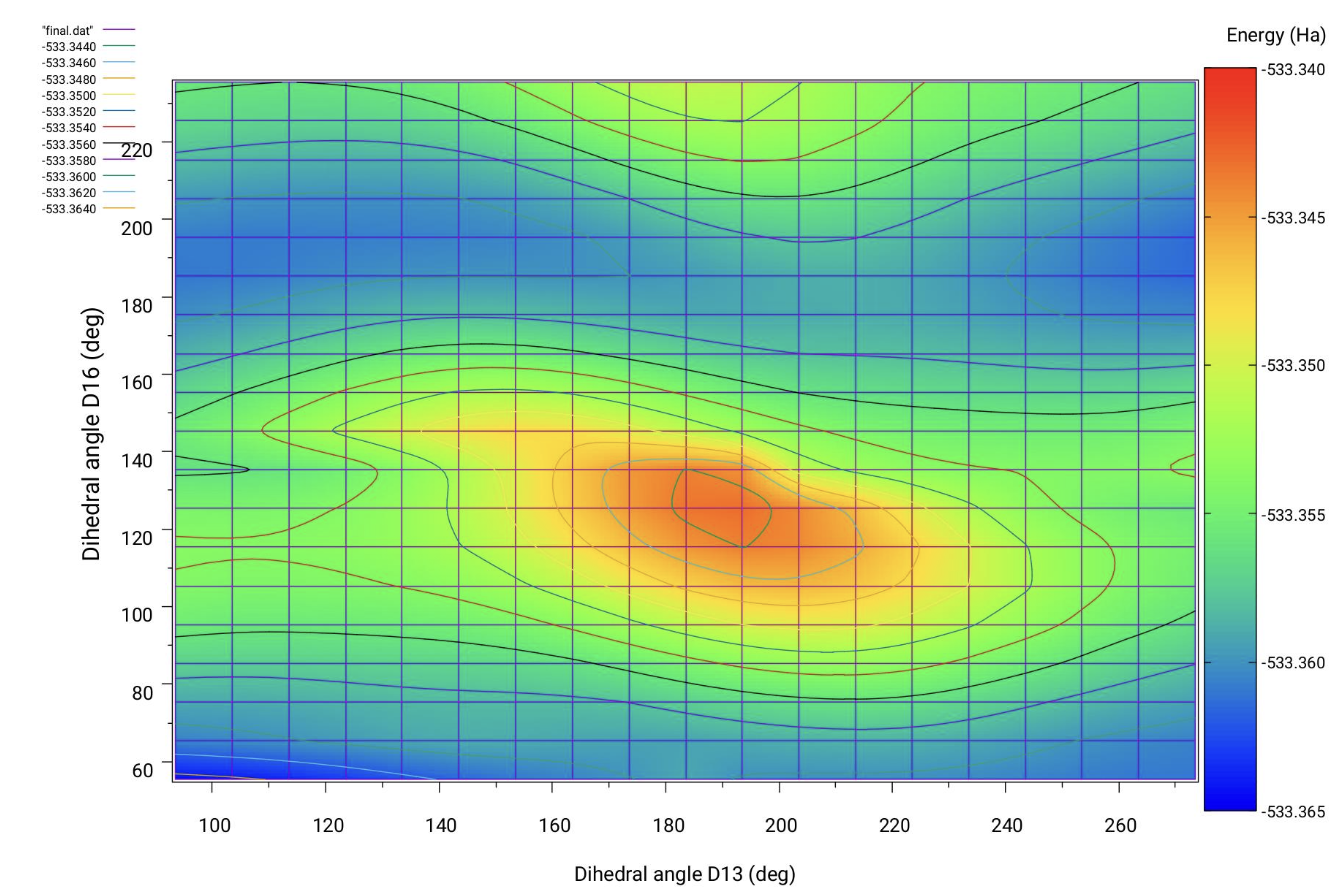
\includegraphics[width=0.7\textwidth]{2dPES.png}
    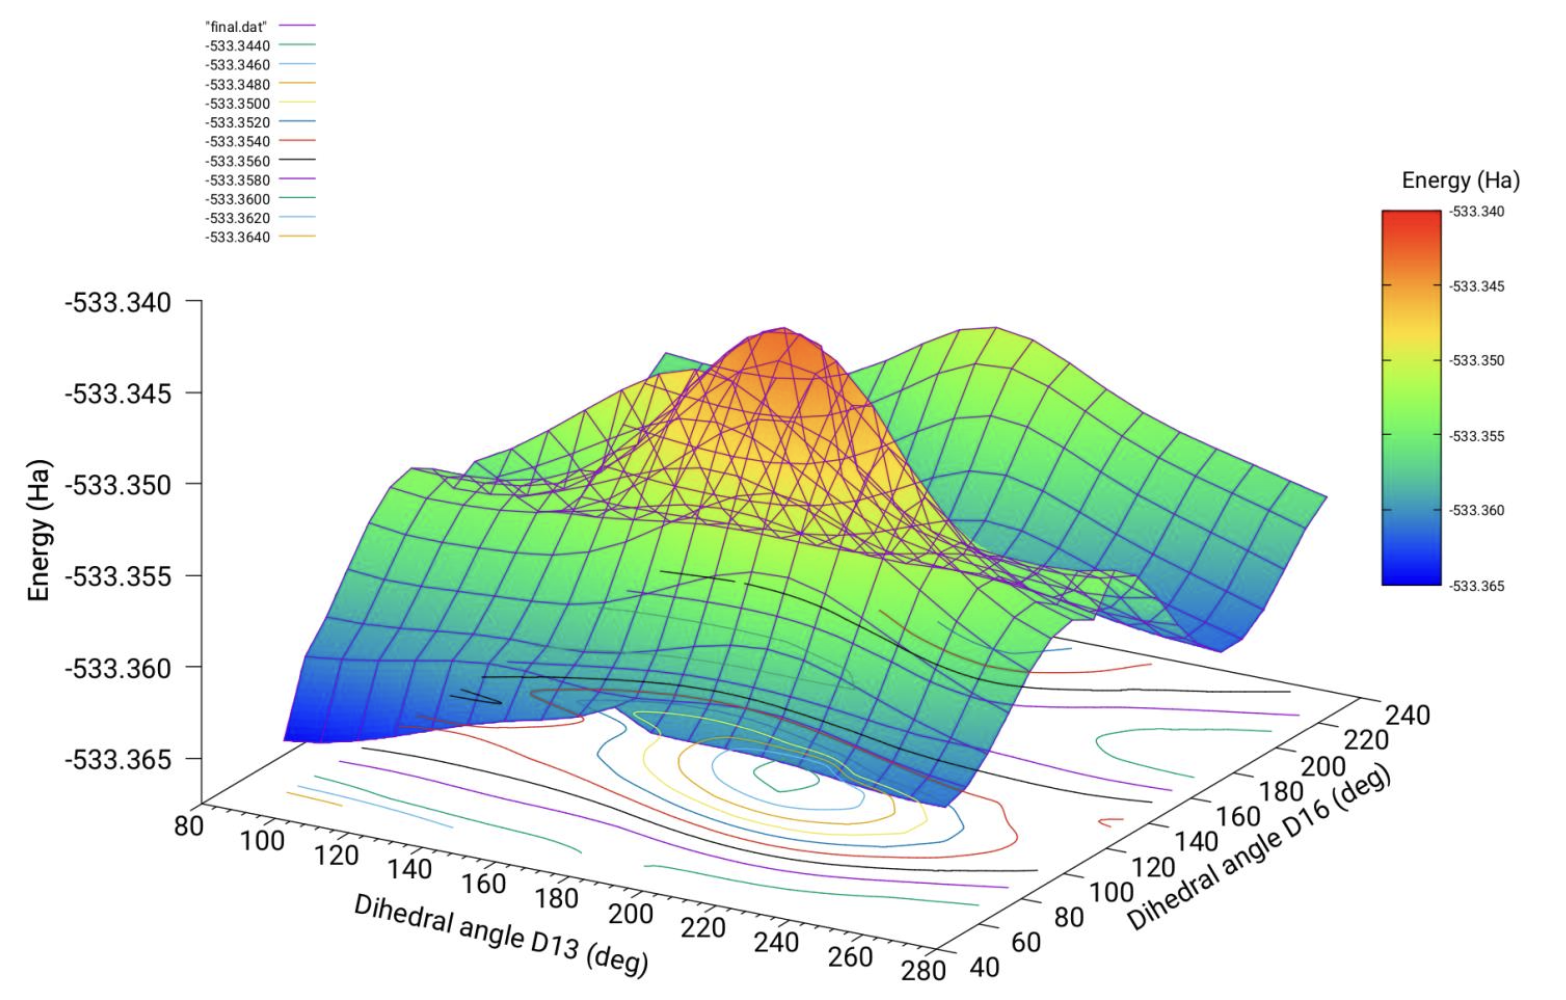
\includegraphics[width=0.7\textwidth]{3dPES.png}
    \caption{2D and 3D-PES plots of hydroxytyrosol}
    \label{fig:2D_3D_plots}
\end{figure}

Note: The x and y-axis ranges in the plots may need adjustment to suit your particular scans. The same applies to the grid settings. In the case of hydroxytyrosol, we opted for 19x19 grid points as they aligned with the scan steps (361 conformers here).

\newpage
\subsection{IR and Raman intensities}

To extract the frequencies, IR and Raman intensities and activities from the Gaussian output file, use the IR$\textunderscore$Raman$\textunderscore$Info.py script. Here, we provide an example for the methanol molecule. 

\begin{itemize}
    \item Run the IR$\textunderscore$Raman$\textunderscore$Info.py script in the directory where your Gaussian output file is located in by typing:
% Python code block
\begin{lstlisting}[style=python]
python3 IR_Raman_Info.py
\end{lstlisting}
    \item You will be required to provide the output filename, laser beam frequency (in cm$^{-1}$), and temperature (in K):
\end{itemize}

\begin{lstlisting}[style=bash]
Enter the filename (e.g., ch3oh.log): 
ch3oh.log
Insert frequency value of laser excitation (cm-1):
18796.99
Insert temperature value (K): (e.g., 298.15 K)
298.15
\end{lstlisting}

The end result is a file called IR\_Raman.csv containing data on IR and Raman intensities and activities.
\begin{table}[h]
\centering
\begin{tabular}{lrrrr}
\hline
 &  &               & Raman & \\ 
 &  & IR intensity & activity & Raman \\
 &    Freq. (cm$^{-1}$)               & (km/mol) & (\AA$^4$/amu) & intensity \\

\hline
$\omega_{1}$ & 538.92 & 123.05 & 2.98 & 3875.50 \\
$\omega_{2}$ & 1114.81 & 83.97 & 9.46 & 4864.03 \\
$\omega_{3}$ & 1169.13 & 39.82 & 1.39 & 670.29 \\
$\omega_{4}$ & 1246.56 & 2.87 & 4.33 & 1930.02 \\
$\omega_{5}$ & 1514.99 & 46.95 & 1.58 & 544.04 \\
$\omega_{6}$ & 1582.79 & 10.85 & 2.98 & 965.53 \\
$\omega_{7}$ & 1597.55 & 2.00 & 14.16 & 4530.13 \\
$\omega_{8}$ & 1606.70 & 2.98 & 14.36 & 4558.60 \\
$\omega_{9}$ & 3169.82 & 57.01 & 144.11 & 15829.67 \\
$\omega_{10}$ & 3230.85 & 87.20 & 73.93 & 7843.97 \\
$\omega_{11}$ & 3291.97 & 44.34 & 80.85 & 8287.83 \\
$\omega_{12}$ & 3976.59 & 46.60 & 69.05 & 4890.86 \\
\hline
\end{tabular}
\label{tab:data_table}
\end{table}

The Raman activities are converted to Raman intensities through the following equation:\cite{Polavarapu1990,Keresztury1993}

\begin{equation}
I_i = \frac{(2\pi)^4}{45}(v_0 - v_i)^4\frac{h}{8\pi^2cv_i(1-exp(-\frac{hv_ic}{kT}))}S_i
\end{equation}

Here, $S_i$, $v_i$, $v_0$, h, c, k, and T represent Raman activities, frequency of the \textit{i}$^{th}$ band, frequency of the incident laser, Planck constant, speed of light, Boltzmann constant, and temperature, respectively.

In addition to that, the spectral data can be plotted in two bar graphs.

\begin{figure}[h] 
    \centering
    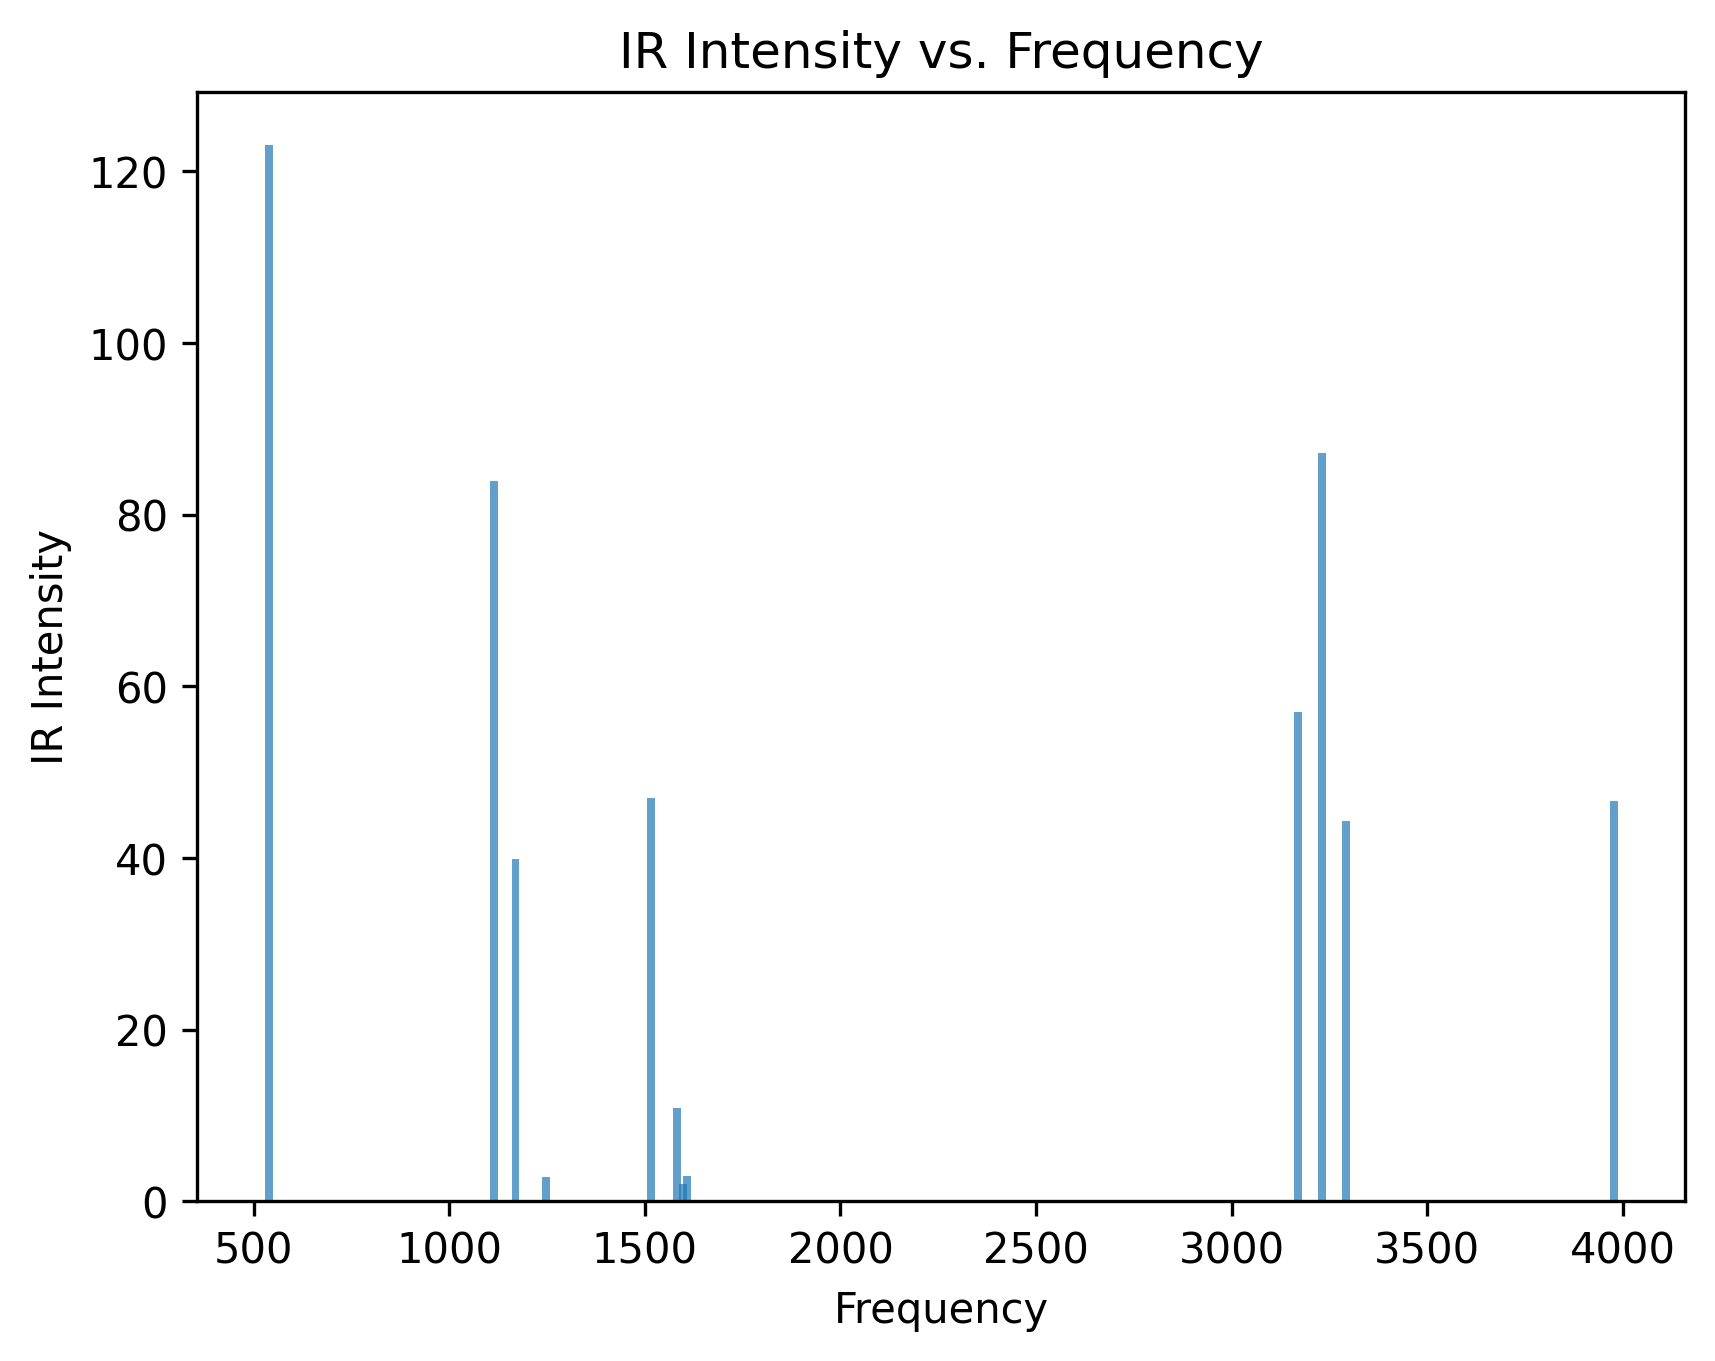
\includegraphics[width=0.6\textwidth]{IR_Intensities.png}
    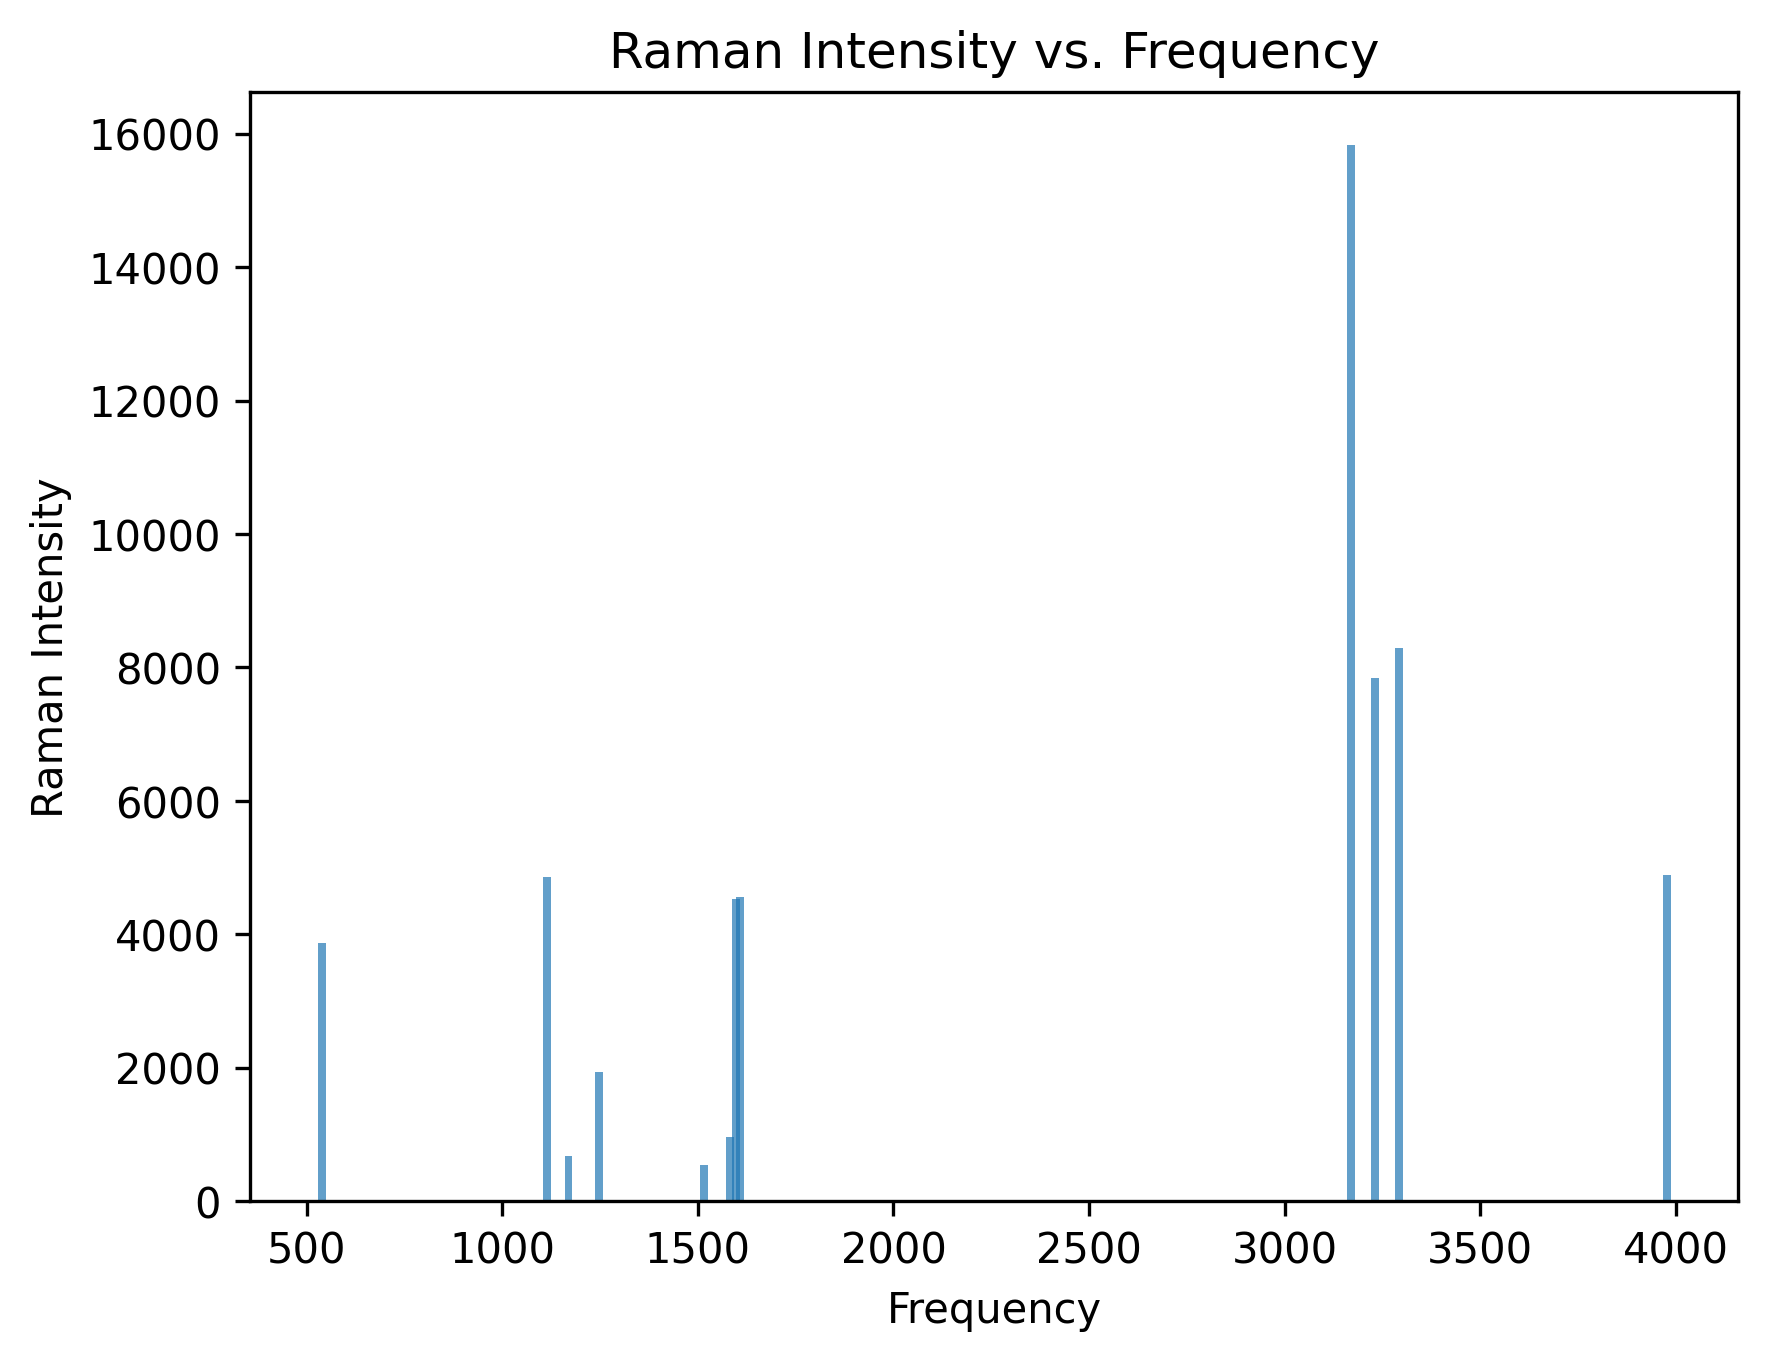
\includegraphics[width=0.6\textwidth]{Raman_Intensities.png}
    \caption{IR and Raman intensities for the methanol molecule}
    \label{fig:ir_intensity}
\end{figure}

\bibliographystyle{plainnat}
\bibliography{argoreferences}
\end{document}



